\documentclass[11pt,a4paper]{article}
\usepackage[margin=22mm]{geometry}
\usepackage{xeCJK,amsmath,amssymb,tikz}
\IfFontExistsTF{Songti SC}{\setCJKmainfont{Songti SC}}{\setCJKmainfont{FandolSong-Regular.otf}}
\usetikzlibrary{arrows.meta,calc,angles,quotes}
\pagestyle{empty}
\setlength{\parindent}{2em}
\setlength{\parskip}{5pt}
\begin{document}
\begin{center}\Large 光滑斜面上的滑块\end{center}
一个小物块从静止开始沿固定的光滑斜面下滑。斜面倾角为 $30^\circ$，物块沿斜面滑行 $2.0\,\mathrm m$，取 $g=10\,\mathrm{m\,s^{-2}}$。求此时物块的速度大小。
\begin{center}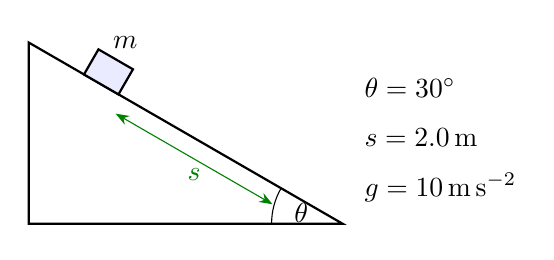
\begin{tikzpicture}[>=Stealth,scale=1.15]
\coordinate (A) at (0,2);\coordinate (B) at (3.464,0);\coordinate (C) at (0,0);
\draw[thick] (A)--(B)--(C)--cycle;
\draw pic[draw,angle radius=9mm,"$\theta$"] {angle=A--B--C};
\begin{scope}[shift={(0.8,1.538)},rotate=-30]
\draw[fill=blue!8,thick] (-.22,0) rectangle (.22,.32);
\node at (0,.53) {$m$};
\draw[<->,green!50!black] (.3,-.2)--(2.3,-.2) node[midway,below] {$s$};
\end{scope}
\node[right] at (3.6,1.5) {$\theta=30^\circ$};
\node[right] at (3.6,.95) {$s=2.0\,\mathrm m$};
\node[right] at (3.6,.4) {$g=10\,\mathrm{m\,s^{-2}}$};
\end{tikzpicture}
\end{center}
物块沿图中的斜边运动，$s$ 是沿斜面的位移。重力竖直向下，支持力垂直斜面。
\begin{center}\begin{tikzpicture}[>=Stealth,scale=1.05]
\draw[thick] (-1,0.577)--(1.5,-.866);
\fill (0,.14) circle (2pt);\node[above right] at (0,.14) {$m$};
\draw[->,red,thick] (0,.14)--(0,-1.3) node[below] {$mg$};
\draw[->,blue,thick] (0,.14)--(.623538,1.22) node[above] {$F_N$};
\draw[->,green!50!black,thick] (0,.14)--(.623538,-.22) node[right] {$mg\sin\theta$};
\draw[dashed] (0,-1.3)--(.623538,-.22);
\node[right] at (1.8,.4) {沿斜面向下为正};
\end{tikzpicture}
\end{center}
沿斜面向下取正方向。重力的切向分量为 $mg\sin\theta$，由牛顿第二定律得
\begin{equation}mg\sin\theta=ma.\label{eq:newton}\end{equation}
约去质量并代入倾角，得到恒定加速度
\begin{equation}a=g\sin\theta=10\times\frac12=5\,\mathrm{m\,s^{-2}}.\label{eq:a}\end{equation}
从静止开始的匀加速运动满足
\begin{equation}s=\frac12at^2\label{eq:s}\end{equation}
\begin{equation}v=at\label{eq:vt}\end{equation}
消去 $t$：
\begin{equation}v^2=a^2t^2=2as.\label{eq:kinematics}\end{equation}
取速度的正值，
\begin{equation}v=\sqrt{2as}=\sqrt{2\times5\times2}=2\sqrt5\,\mathrm{m\,s^{-1}}.\label{eq:v}\end{equation}
沿斜面的重力分量决定加速度，再由滑行距离决定末速度。在这个固定光滑斜面上，质量约去，相同起点释放的物块具有相同的加速度。
\end{document}
